% Architecture + where the instrument reads. PAPER_BRIEF §8.2 asks for this to be
% schematic rather than a literal layer-by-layer box diagram: the point is not
% the MLP (which is unremarkable) but *where the two probe batches enter* and
% *when recycling fires relative to task boundaries*.
\begin{figure}[t]
\centering
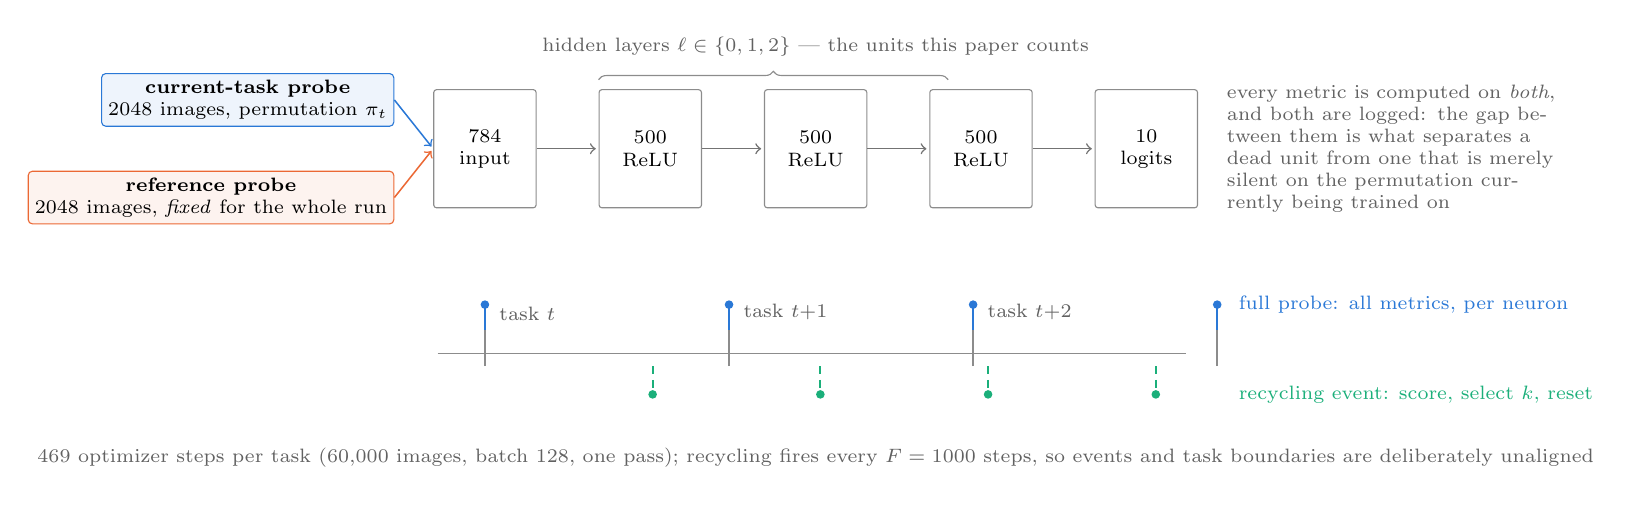
\begin{tikzpicture}[
  font=\small,
  layer/.style = {draw=black!45, rounded corners=1pt, minimum width=13mm,
                  minimum height=15mm, align=center, font=\scriptsize, fill=white},
  probe/.style = {draw=#1, rounded corners=1.5pt, fill=#1!8, align=center,
                  font=\scriptsize, inner sep=2.4pt},
  sub/.style   = {font=\scriptsize, text=black!62},
  ar/.style    = {->, black!55, line width=0.55pt, shorten >=1pt},
]
\definecolor{cCur}{HTML}{2A78D6}
\definecolor{cRef}{HTML}{EB6834}
\definecolor{cEv}{HTML}{1BAF7A}

% ---- the network -------------------------------------------------------------
\node[layer] (in)  at (0,0)   {$784$\\input};
\node[layer] (h1)  at (2.1,0) {$500$\\ReLU};
\node[layer] (h2)  at (4.2,0) {$500$\\ReLU};
\node[layer] (h3)  at (6.3,0) {$500$\\ReLU};
\node[layer] (out) at (8.4,0) {$10$\\logits};
\foreach \a/\b in {in/h1, h1/h2, h2/h3, h3/out} \draw[ar] (\a) -- (\b);

\node[sub, anchor=south] at (4.2,1.05)
  {hidden layers $\ell \in \{0,1,2\}$ --- the units this paper counts};
\draw[decorate, decoration={brace, amplitude=3pt}, black!45]
  (h1.north west) ++(0,0.12) -- ++(4.44,0);

% ---- the two probe batches ---------------------------------------------------
\node[probe=cCur, anchor=east] (pc) at (-1.15,0.62)
  {\textbf{current-task probe}\\$2048$ images, permutation $\pi_t$};
\node[probe=cRef, anchor=east] (pr) at (-1.15,-0.62)
  {\textbf{reference probe}\\$2048$ images, \emph{fixed} for the whole run};
\draw[ar, cCur] (pc.east) -- (in.west);
\draw[ar, cRef] (pr.east) -- (in.west);
\node[sub, anchor=west, text width=42mm] at (9.3,0)
  {every metric is computed on \emph{both}, and both are logged: the gap between
   them is what separates a dead unit from one that is merely silent on the
   permutation currently being trained on};

% ---- the training timeline ---------------------------------------------------
\def\ty{-2.6}
\draw[black!45, line width=0.6pt] (-0.6,\ty) -- (8.9,\ty);
\foreach \x/\lab in {0/{task $t$}, 3.1/{task $t{+}1$}, 6.2/{task $t{+}2$}}{
  \draw[black!45, line width=0.9pt] (\x,\ty-0.16) -- (\x,\ty+0.30);
  \node[sub, anchor=south west] at (\x+0.06,\ty+0.30) {\lab};
}
\draw[black!45, line width=0.9pt] (9.3,\ty-0.16) -- (9.3,\ty+0.30);
\node[sub, anchor=north] at (4.2,\ty-1.08)
  {$469$ optimizer steps per task ($60{,}000$ images, batch $128$, one pass);
   recycling fires every $F=1000$ steps, so events and task boundaries are
   deliberately unaligned};

% probe read-outs at boundaries
\foreach \x in {0, 3.1, 6.2, 9.3}{
  \draw[cCur, line width=0.7pt] (\x,\ty+0.30) -- (\x,\ty+0.62);
  \node[circle, fill=cCur, inner sep=1.1pt] at (\x,\ty+0.62) {};
}
\node[sub, anchor=west, text=cCur] at (9.45,\ty+0.62) {full probe: all metrics, per neuron};

% recycling events
\foreach \x in {2.13, 4.26, 6.39, 8.52}{
  \draw[cEv, line width=0.7pt, densely dashed] (\x,\ty-0.16) -- (\x,\ty-0.52);
  \node[circle, fill=cEv, inner sep=1.1pt] at (\x,\ty-0.52) {};
}
\node[sub, anchor=west, text=cEv] at (9.45,\ty-0.52) {recycling event: score, select $k$, reset};

\end{tikzpicture}
\caption{\textbf{Setting and instrument.} A $784$--$500$--$500$--$500$--$10$
ReLU MLP on online permuted MNIST: each task is a fresh input permutation seen
for a single pass, and the outcome measure is online accuracy, scored on the
forward pass taken \emph{before} each update. Every death metric is evaluated on
two probe batches --- the current task's distribution and a reference
distribution fixed for the entire run --- and per-neuron state is written at
every task boundary. Recycling events are governed by an optimizer-step counter
($F=1000$) rather than by task index, so they fall inside tasks rather than at
their edges.}
\label{fig:arch}
\end{figure}
